\subsection{Demonstration} \label{subsection:demonstration}

For Gatchina, a polycentric master plan was proposed.
Instead of expanding the city through mass housing on the periphery, the approach strengthens existing centers and improves the provision of basic services within residential blocks.
This aligns with the concept of sustainable urban development.
According to existing protected zones, the model preserves Gatchina’s historic park core, while also accounting for view corridors and the continuity of the green infrastructure network.
Existing business blocks are proposed to be strengthened, while residential blocks are supplemented with social infrastructure to ensure access to essential services.
The master plan strategy is based on the conducted analysis, which revealed a spatial mismatch between residential locations and basic services.
The city has a strong transport block with a railway hub; the model proposes reinforcing peripheral interchange nodes as transport blocks \ref{figure:priority}.
The proposals take into account the city’s current needs and may serve as a basis for a real-world master plan.

\begin{figure}
    \centering
    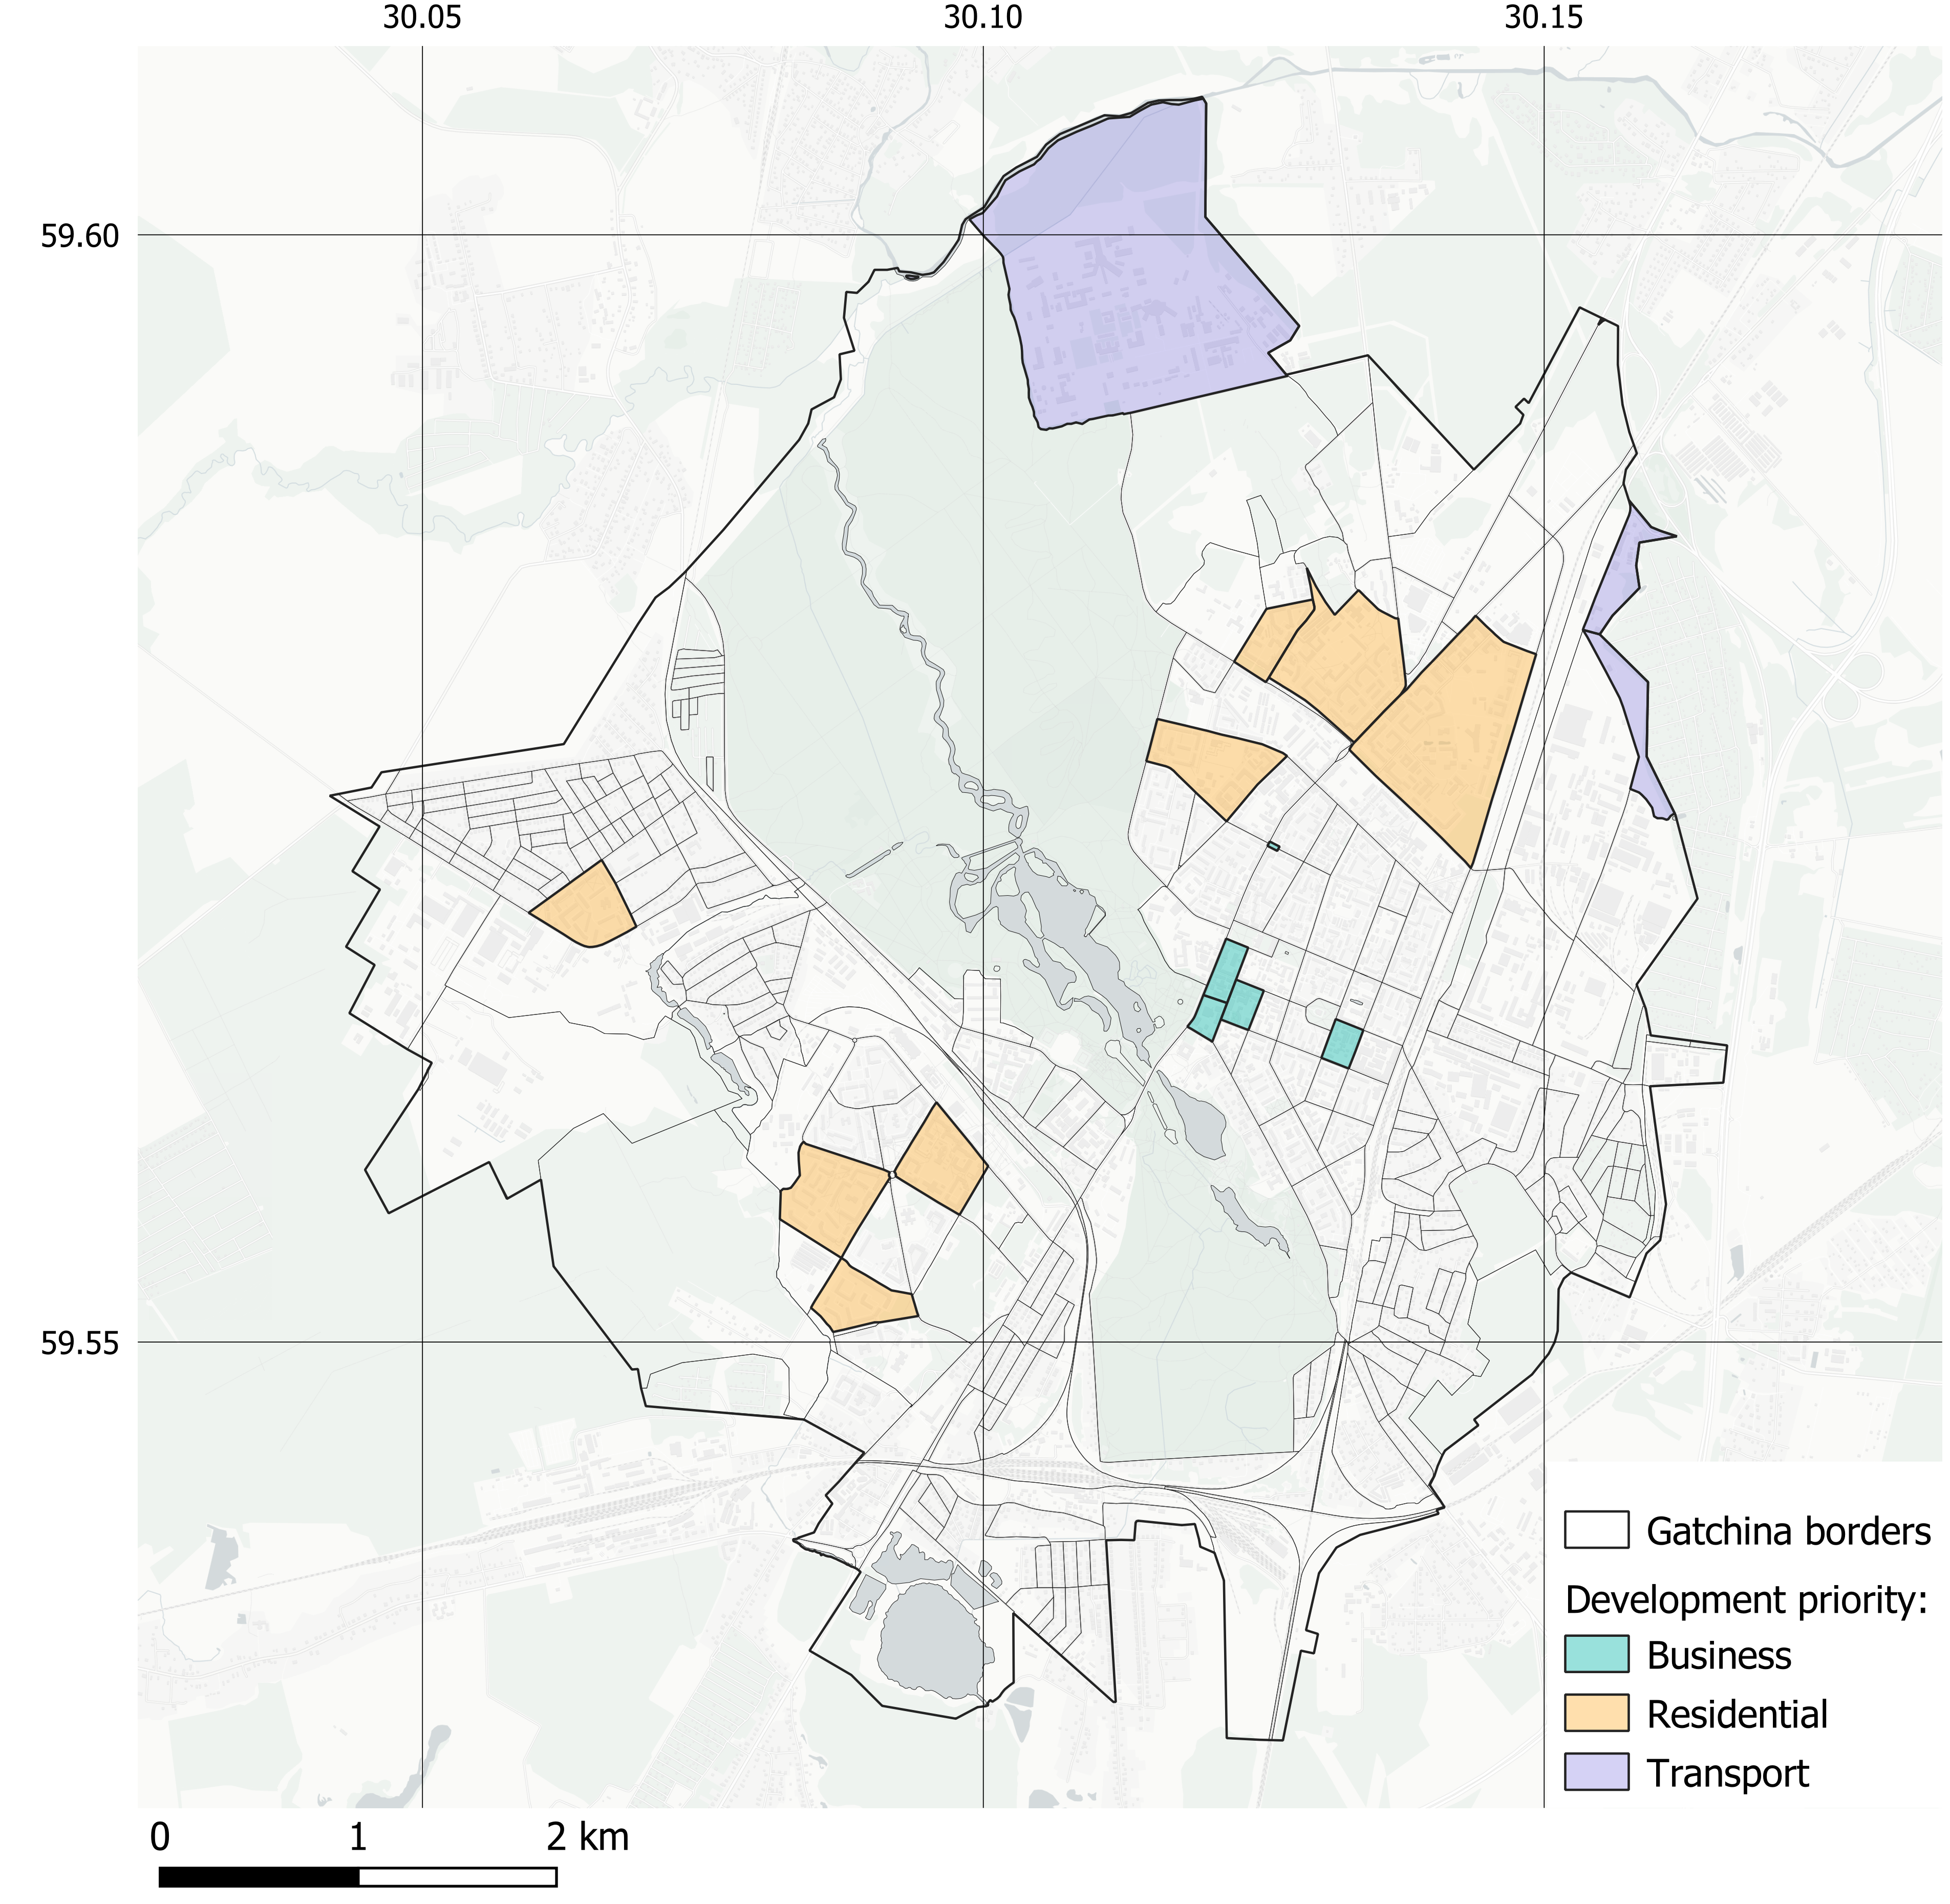
\includegraphics[width=0.85\linewidth]{Sections/5_results/Figures/development_priority.png}
    \caption{Development priority}
    \label{figure:priority}
\end{figure}

\subsubsection{Run Overview}

The run was executed on the base gpt-5.5 model with a limit of seven iterations; total runtime was approximately 44 minutes.
The system performed exactly 300 tool calls, involving four executor agents, an orchestrator, and a critic.
The distribution of calls is strongly asymmetric (see Table \ref{table:case_agent_load}): 237 out of 300 (79\%) were performed by BlocksNet agent, while textual agents (WebSearch, Normative) operated in limited bursts.
Importantly, on this ill-defined brief, cooperation did not collapse after the initial coverage of subqueries: computational executors were repeatedly reassigned, and the critic injected an additional round.
In other words, the system generated \emph{deep} cooperation that matched the task complexity, exhibiting the behavior this case study was designed to observe.

\begin{table}[h]
\centering
\small
\begin{tabular}{lccl}
\hline
\textbf{Agent} & \textbf{Calls} & \textbf{Share} & \textbf{Work profile} \\
\hline
BlocksNet    & 237 & 79.0\% & Block-level model diagnostics + development scenarios \\
WebSearch    & 38  & 12.7\% & Socio-economic profiling, web search / URL reading \\
CodeSpatial  & 14  & 4.7\%  & OSM-based geocomputation, executable Python \\
Normative    & 11  & 3.7\%  & Regulatory corpus search, protected status analysis \\
\hline
\textbf{Total} & \textbf{300} & \textbf{100\%} & \\
\hline
\end{tabular}
\caption{Agent load in the case study (number of tool calls in the log).}
\label{table:case_agent_load}
\end{table}

\subsubsection{BlocksNet Agent: Domain Executor}

The main executor was \textbf{BlocksNetAgent}.
Unlike the three general-purpose tool agents, it is specialized in spatial-quantitative diagnostics and includes a suite of more than thirty tools organized into a stable pipeline: 

\begin{enumerate}
    \item \emph{discovery}:
    \begin{itemize}
        \item \texttt{list\_service\_types},
        \item \texttt{list\_key\_services},
        \item \texttt{list\_cached\_data}.
    \end{itemize}
    \item \emph{loading}:
    \begin{itemize}
        \item \texttt{load\_blocks},
        \item \texttt{load\_accessibility\_matrix}.
    \end{itemize}
    \item \emph{computation}:
    \begin{itemize}
        \item \texttt{compute\_mean\_accessibility},
        \item \texttt{compute\_service\_provision},
        \item \texttt{compute\_services\_centrality},
        \item \texttt{compute\_population\_centrality},
        \item \texttt{compute\_density\_indicators},
        \item \texttt{compute\_shannon\_diversity},
        \item \texttt{compute\_connectivity}.
    \end{itemize}
    \item \emph{retrieval}:
    \begin{itemize}
        \item \texttt{get\_analysis\_results},
        \item \texttt{get\_block\_info}
    \end{itemize}
    \item \emph{scenario}:
    \begin{itemize}
        \item \texttt{suggest\_target\_blocks},
        \item \texttt{propose\_zone\_development},
        \item \texttt{compute\_scenario\_provision}.
    \end{itemize}
\end{enumerate}

It is precisely the breadth of this toolset and the block-level granularity (77 calls to \texttt{get\_block\_info}, 54 to \texttt{get\_analysis\_results}) that explain its 79\% share of all calls.

The agent’s reasoning is structured as a reproducible scheme:

\begin{enumerate}
    \item \texttt{ANALYSIS PLAN}: the agent relies on working cards 
      (masterplan baseline workflow, accessibility network, services diversity and density, land use optimization, and service gap workflow), formulates information needs, and justifies each tool selection ("\texttt{compute\_services\_centrality} 
      and \texttt{compute\_population\_centrality} to separate service centers from population-dense quarters").
    
    \item \texttt{REFLECTION}: the agent aggregates and cross-validates results.
    
    \item \texttt{HYPOTHESES}: the agent formalizes testable claims in a 
      \emph{claim / test / verdict} format ("claim: adding capacity improves 
      provision; test: \texttt{compute\_scenario\_provision}; verdict: supported"). 
      The agent itself defines the logic: "first measure the baseline state of 
      the city, then propose a testable development hypothesis."
    
    \item \texttt{RESULT}: the agent generates final output from the previous steps.
\end{enumerate}

\subsubsection{Adaptive Collaboration Depth}

The log reflects not a single task allocation but iterative reassignment of executors. Grouping the 300 calls into consecutive single-agent segments yields 17 dispatch segments (see Figure \ref{figure:case_collab}).
The run begins with a short capability check (CodeSpatial queries available libraries), followed by alternating limited WebSearch and Normative bursts for context collection and large BlocksNet segments (18, 37, 50, 32, 54, 46 calls), into which model-driven diagnostics return six times as the task is progressively refined.

\begin{figure}[h]
    \centering
    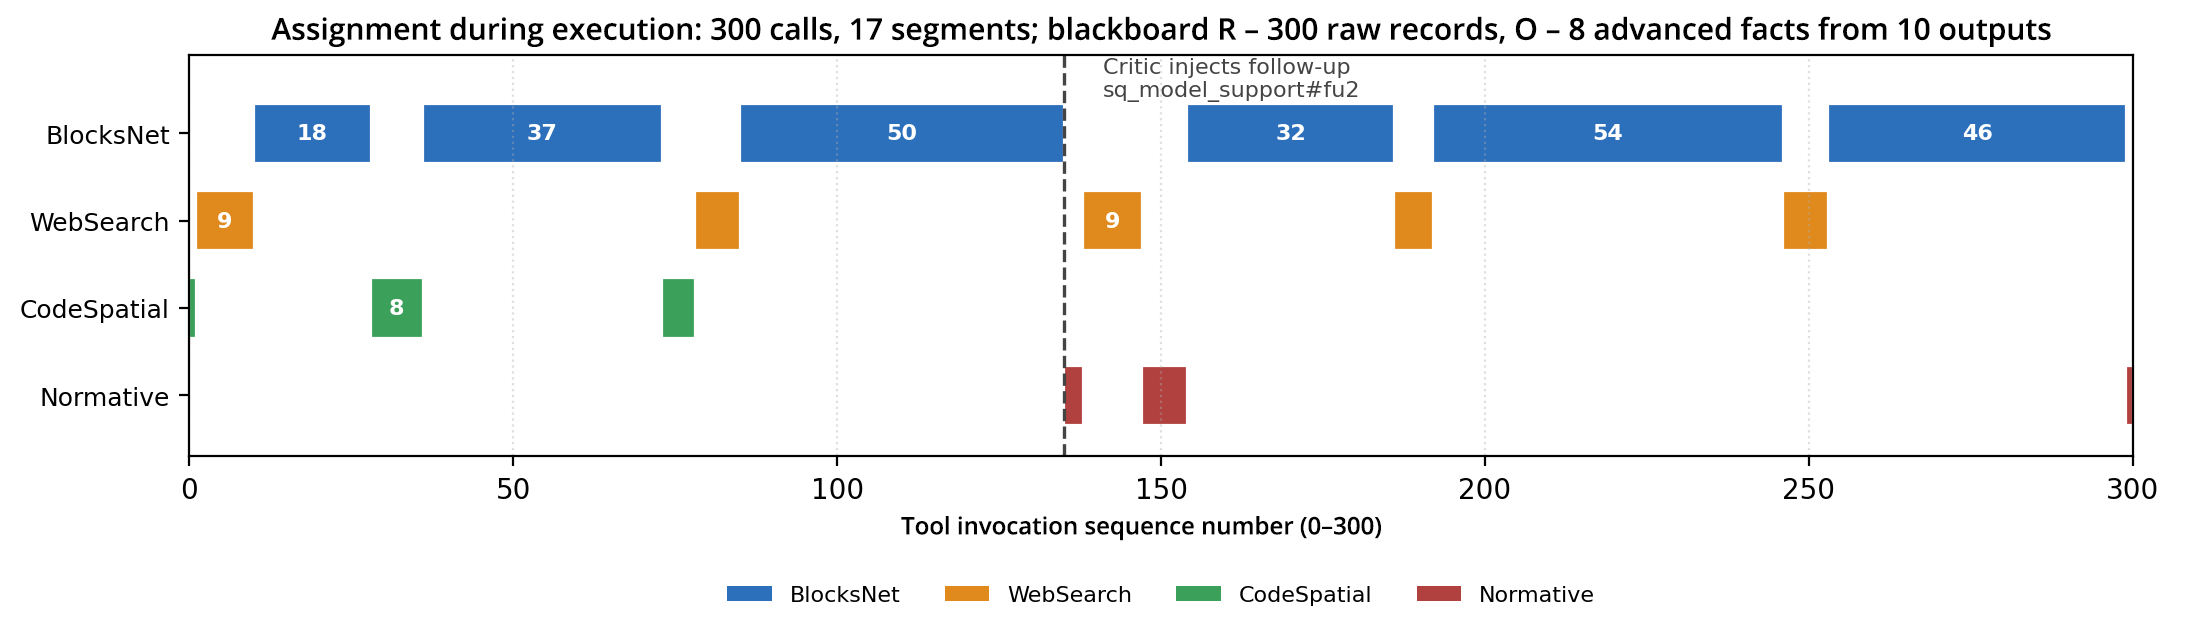
\includegraphics[width=1.0\linewidth]{Sections//5_results//Figures/case_collaboration_timeline.png}
    \caption{Dispatcher timeline of executors over 300 tool calls (17 segments). BlocksNet returns to execution six times; WebSearch/Normative provide limited context bursts. The dashed line indicates the point after which the critic injected follow-up \texttt{sq\_model\_support\#fu2}; this is followed by the second half of BlocksNet segments. The blackboard accumulates 300 raw records ($R$), of which 10 structured outputs from executors result in 8 promoted factual statements ($O$).}
    \label{figure:case_collab}
\end{figure}

A key episode of collaboration is the injection of an additional round.
After identifying in \texttt{REFLECTION} a mismatch between the service center (block 136) and the population center (block 331), the system opened follow-up \texttt{sq\_model\_support\#fu2}, targeting precisely this uncovered aspect; five of ten structured outputs and the entire second half of BlocksNet segments in Figure \ref{figure:case_collab} are associated with this step.
This illustrates adaptive depth: a well-posed query would have been completed in a single pass, whereas this ill-defined brief triggers additional rounds autonomously.
Other mechanisms (routing, curation, mediator, critique) are only visible through their effects-reassignment, injection, and promotion of results.

\subsubsection{Tool-Grounded Evidence and Context Integration}

All reported figures are produced via tool execution rather than model priors.
BlocksNet recorded in \texttt{REFLECTION}/\texttt{RESULT} an average accessibility of 45.59 minutes (best block 196: 32.67 min; worst block 285: 72.01 min) and systemic 15-minute service deficits: clinics --- 0.295 (332 out of 351 blocks underserved), supermarkets --- 0.288, stadiums --- 0.152, local shops --- 0.296, while schools --- 0.774, pharmacies --- 0.821, and stops --- 0.962.
Service centrality concentrates in block 136 (0.8037), while population centrality peaks in block 331 (1.000); this discrepancy triggered the follow-up.
The development scenario (pipeline \texttt{suggest\_target\_blocks} $\rightarrow$ \texttt{propose\_zone\_development} $\rightarrow$ \texttt{compute\_scenario\_provision}) for blocks [2, 9, 18, 87, 89, 108, 289, 331] was validated via a before/after comparison: clinics 0.295 $\rightarrow$ 0.833 (fully served blocks 13 $\rightarrow$ 86), schools 0.774 $\rightarrow$ 0.898, pharmacies 0.821 $\rightarrow$ 0.900, sports facilities 0.460 $\rightarrow$ 0.545.

Context was provided by other agents: Normative, via web search, established the protected status (the palace and park ensemble as part of a UNESCO object) and SP 42.13330 service radius standards; CodeSpatial extracted the transport framework from OpenStreetMap via the mandatory chain \texttt{HYPOTHESIS} $\rightarrow$ $\dots$ $\rightarrow$ \texttt{INTERPRET} (Figure \ref{figure:case_transport}); WebSearch collected socio-economic profiles.
Only reliable findings are promoted to the shared board: BlocksNet outputs and the completed CodeSpatial transport analysis \texttt{sq\_003} (confidence 0.78) are marked \emph{promoted}, while incomplete code attempts \texttt{sq\_002}/\texttt{sq\_model\_support} (confidence 0.30) remain \emph{not promoted} --- 8 out of 10 structured outputs pass the gating mechanism.
The observed threshold aligns with the promotion rule, and low confidence is explicitly justified by the agent itself (“numeric self-check missing”, “final text did not expose a RESULT field with numbers”).

The run also demonstrates robustness to source degradation: WebSearch requests to \texttt{ru.wikipedia.org} returned 403 Forbidden, several Normative URLs were broken, and an Overpass query from CodeSpatial was rejected by the server.
None of these failures interrupted execution: the system continued using available snippets while preserving a tool-verifiable core.
Additionally, an executable-code safeguard triggered a static Pyflakes check (F401) that blocked \texttt{run\_validated\_python} before execution.

\begin{figure}[h]
    \centering
    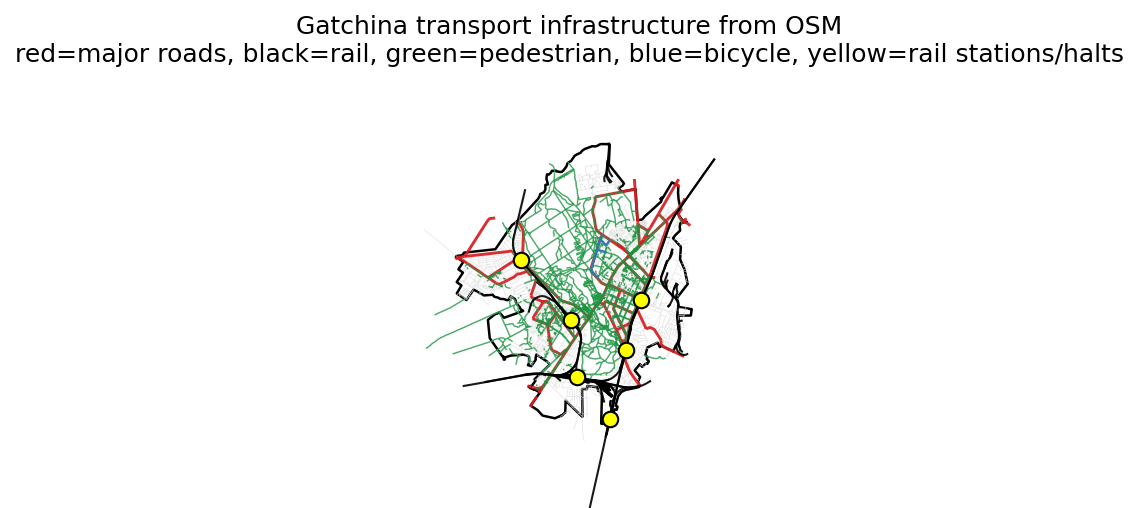
\includegraphics[width=0.62\linewidth]{Sections//5_results//Figures/gatchina_transport_osm.png}
    \caption{Transport network of Gatchina extracted by CodeSpatial from OpenStreetMap (subquery \texttt{sq\_003}).}
    \label{figure:case_transport}
\end{figure}

\begin{figure}[h]
    \centering
    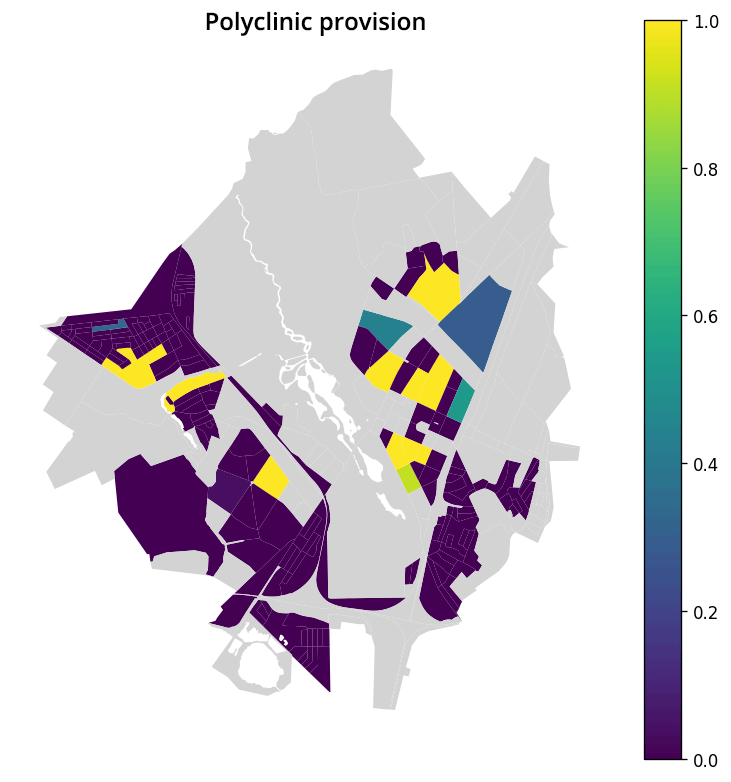
\includegraphics[width=0.62\linewidth]{Sections//5_results//Figures/competitive_provision_polyclinic.png}
    \caption{Clinic provision map by block (BlocksNet): strong provision 0.295, with 332 out of 351 blocks underserved. The deficit was identified via \texttt{compute\_service\_provision}.}
    \label{figure:case_polyclinic}
\end{figure}

\subsubsection{Generated Artifacts}

The system produces inspectable and reusable outputs, not only text: 71 saved artifacts including 34 CSV tables (block-level service provision, scenario deltas), 19 maps (provision, accessibility, centrality, diversity, density), 7 web-sourced images, and one generated transport network figure.
The transport network (Figure~\ref{figure:case_transport}) and clinic provision map (Figure~\ref{figure:case_polyclinic}) are the most illustrative, as both directly correspond to key evidence.

\subsubsection{Limitations and Threats to Validity}

To avoid overinterpreting a single case, we note the following:

\begin{itemize}
  \item This analysis involves a single task, a single base model, and a single run. As such, it should be regarded as an illustration of a coordination mechanism rather than a statistical proof. The demonstration of adaptive depth is based on one complex brief, with no paired simple baseline case for comparison.
  \item The reasoning chain is constrained by the local BlocksNet model, which includes no up-to-date budgets, land ownership, infrastructure networks, or legal constraints. Furthermore, the optimizer is stochastic, meaning scenario outputs are model-based hypotheses.
  \item Some external requests failed: 403 Forbidden, broken URLs, and rejected Overpass queries. The system degraded gracefully, but the completeness of web and OSM context is reduced.
  \item Behavior is observed through execution logs. Internal orchestrator and critic messages are reconstructed from effects (reassignment, follow-up \texttt{\#fu2}, promotion status), not from a verbatim transcript.
\end{itemize}
